\section{Grundlagen}
\subsection{Wichtige Formeln}
    \begin{longtable}{| p{.25\textwidth} | p{.40\textwidth} | p{.30\textwidth} |}
        \firsthline
        \textbf{Elektrische Kraft} \newline
        \tabbild[width=3.5cm]{images/ElKraft.png}  &
        \begin{equation*}\vec{F_e} = \dfrac{1}{2\pi\epsilon}\cdot\dfrac{Q\cdot q}{r}\cdot\vec{r_0}\end{equation*}
        \begin{equation*}F_e = \dfrac{\pi\cdot U^2}{2\cdot r\cdot(\ln{\dfrac{r-R_1}{R_1}})^2}\end{equation*} & \newline
        [${F_e}$] = $\dfrac{N}{m}$\newline \newline 
        $\epsilon\;\widehat{=}\;$elektrische Permittivität\newline 
        $\epsilon_0 = 8.8542 \cdot 10^{-12}$ $\left[\dfrac{As}{Vm}\right]$ \newline \newline
        Q,q$\,\widehat{=}\,$Linienladungsdichte$\,\left[\dfrac{C}{m}\right]$ 
        \\ \hline
        
        \textbf{Magnetische Kraft} \newline
        \tabbild[width=3.5cm]{images/magnetischeKraft.png}  &	
        \begin{equation*}\vec{F_m} = \dfrac{\mu}{2\pi}\cdot\dfrac{I\cdot i}{r}\cdot\vec{r_0}\end{equation*} 
        \begin{equation*}F_m = \dfrac{\mu_0\cdot I^2}{2\cdot\pi\cdot r}\end{equation*} 
        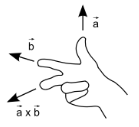
\includegraphics[width=3cm]{images/vektorprodukt.png}	& \newline
        $\mu$ $\widehat{=}$ magnetische Permeabilität\newline 
        $\mu_0$ = $4\pi\cdot 10^{-7} \,\left[\dfrac{N}{A^2}\right]=\left[\dfrac{Vs}{Am}\right]$ \newline \newline
        $\vec{r_0}=\dfrac{\vec{r}}{|\vec{r}|}$ \newline \newline 
        I, i $\widehat{=}$ elektrische Ströme 	\newline \newline 
        $[F_m]$ = $\dfrac{N}{m}$
        \\ \hline
        
        \textbf{Elektrisches Feld} \newline \newline
        \tabbild[width=4cm]{images/elektrischesFeld.png} &
        \begin{equation*}\vec{E} = \dfrac{\vec{F_e}}{q} = \dfrac{1}{2\pi\epsilon}\cdot\dfrac{Q}{r}\cdot\vec{r_0}\end{equation*} 
        \begin{equation*}\vec{E} = \dfrac{1}{2\pi\epsilon}\cdot\dfrac{Q}{r}\cdot\vec{r_0}\end{equation*} & 
        \begin{equation*}[E] = \dfrac{V}{m}\end{equation*} 									
        \\ \hline
        
        \textbf{Elektrisches Potential}  &
        \begin{equation*}\varphi = \int\vec{E}\cdot\vec{dl}	\end{equation*}	& 
        \begin{equation*}[\varphi] = V\end{equation*} 
        \\ \hline
        
        \textbf{Elektrische Spannung}   &
        \begin{equation*}U_{AB} = \int\limits_{A}^{B}\vec{E}\cdot\vec{dl} = \varphi_A - \varphi_B\end{equation*}  & 
        \begin{equation*}[U] = V \end{equation*}  
        \\ \hline
              
        \textbf{Elektrischer Strom} 	    &  
        \begin{equation*}I = \dfrac{dQ}{dt}	\end{equation*} &  
        \begin{equation*}[I] = A\end{equation*} 
        \\ \hline
        		
        \textbf{Magnetische Feldstärke} \newline \newline
        \tabbild[width=4cm]{images/magnetischesFeld.png} &
        \begin{equation*}\vec{H} = \dfrac{I}{2\pi}\cdot\dfrac{\vec{L_0}\times\vec{r_0}}{r} \end{equation*} & 
        \newline [H] = $\dfrac{A}{m}$ \newline
        $\vec{L_0},\vec{l_0}$ $\widehat{=}$ Einheitsvektoren der Stromleiter
        \\ \hline
        
        \textbf{Magnetische Flussdichte}  &
        \begin{equation*}\vec{B} = \mu\cdot\vec{H} = \mu_0\cdot\mu_r\cdot\vec{H}\end{equation*} &  
        \begin{equation*}[B] = T=\dfrac{Vs}{m^2}\end{equation*} 
        \\ \hline
        
        \textbf{Magnetische Fluss} \newline
        \tabbild[width=3.5cm]{images/magnetischeFluss} & 
        \begin{equation*}\phi = \iint\limits_{(A)}\vec{B}\cdot\vec{dA}\end{equation*} &  
        \begin{equation*}[\phi] = Vs = Wb\end{equation*}
        \\ \hline
        
        \textbf{Verkettete Fluss}\newline 
        \tabbild[width=4cm]{images/Verkettetefluss}		 &
        \begin{equation*}\psi = N\cdot\phi\end{equation*}
        \begin{equation*}\psi = L\cdot I\end{equation*}
        \centering\textbf{meistens} 
        \begin{equation*}\psi(t) = N\cdot\iint\limits_{(A)}\vec{B}\cdot\vec{dA}=N\cdot B \cdot A \cdot cos\left(\omega t\right)\end{equation*} & 
        \begin{equation*}[\psi] = Vs = Wb\end{equation*}
        \\ \hline
        
        \textbf{Induzierte Spannung} 	 &
        \begin{equation*}U_{ind} = -\dfrac{d\psi}{dt}=-N\dfrac{d\phi}{dt}\end{equation*}			
        \centering\textbf{meistens} 
        \begin{equation*}U_{ind} = -\dfrac{d\psi}{dt}=\omega\cdot N\cdot B\cdot A\cdot sin\left(\omega t\right)\end{equation*}  &
        \\ \hline
        
        \textbf{Magnetische Durchflutung} \newline \newline
        \tabbild[width=4cm]{images/Durchflutungssatz.png}  &
        \begin{equation*}	 \Theta = \sum\limits_{k=1}^{n}I_k = \oint\limits_{(C)}\vec{H}\cdot\vec{dl}\end{equation*}  
        \centering\textbf{Beispiel:}\
        \begin{equation*}	\oint\limits_{(C)}\vec{H}\cdot\vec{dl} = \int \limits_{P_1}^{P_2}\vec{H}\cdot\vec{dl} + \int \limits_{P_2}^{P_3}\vec{H}\cdot\vec{dl}	+ ... + \int \limits_{P_{m-1}}^{P_m}\vec{H}\cdot\vec{dl}\end{equation*}				&
        \begin{equation*}[\Theta] = A\end{equation*} 
        \\ \hline
        
        \textbf{Magnetische Spannung}	 & 
        \begin{equation*}V_m = \int\limits_{A}^{B}\vec{H}\cdot\vec{dl}\end{equation*}											
        & \begin{equation*}[V_m] = A\end{equation*} 
        \\ \hline 
        
        \textbf{Magnetkreis}	\newline
        \tabbild[width=4cm]{images/magnetkreis.png}  &
        \begin{equation*}\oint\limits_{(C)}\vec{H}\cdot\vec{dl} \approx H\cdot L = N\cdot I\end{equation*}  
        \begin{equation*}\Rightarrow H = \dfrac{N\cdot I}{L}\end{equation*} 
        \begin{equation*}\Rightarrow B = \mu_0\cdot\dfrac{N\cdot I}{L}\end{equation*} &    
        falls L $>>$ R und \newline 
        das Feld in der Spule \textbf{homogen} ist
        \\ \hline
        
        \textbf{Reluktanzkraft} \newline
        \tabbild[width=3.5cm]{images/reluktanzkraft.png} &
        \begin{equation*}F_R = -\dfrac{\partial W_m}{\partial\delta} = \mu_0\cdot\dfrac{N^2\cdot I^2\cdot A_{Fe}}{4\cdot\delta^2}\end{equation*} & 
        wobei $A_{Fe}$ die magnetisch wirksame Fläche des Luftspalts ist. 
        \\ \hline
        \textbf{magnetische Energie} & 
        $W_m = \dfrac{1}{2}\cdot H_\delta\cdot B_\delta\cdot2\cdot A_{Fe}\cdot\delta = \mu_0\cdot \dfrac{I^2\cdot N^2}{4\cdot\delta}\cdot A_{Fe}$
        & wobei $A_{Fe}\cdot\delta$ dem Volumen des Luftspalts entspricht. \\
        \hline
        \textbf{Elektrische Kraft vs.} & \begin{equation*}
        F_e\, = \dfrac{\pi\cdot\epsilon_0\cdot U^2}{2\cdot r\cdot\left(ln\dfrac{r-R_1}{R_1}\right)^2} = 2.88\cdot 10^{-11} \quad \left[\dfrac{N}{m}\right]
        \end{equation*} & Die magnetische Kraft pro Länge \& Strom ist $7 \cdot 10^4$ grösser als die Elektrische Kraft. Daher basieren alle elektrischen Maschinen auf der Magnetische Kraft. \\
        \textbf{Magnetische Kraft}&\begin{equation*}
        F_m = \dfrac{\mu_0\cdot I^2}{2\cdot\pi\cdot r} = 2.00 \cdot 10^{-6} \quad\left[\dfrac{N}{m}\right]
        \end{equation*}&\\    
        \hline    
        \end{longtable}
    \clearpage
